\documentclass{article}
\usepackage[utf8]{inputenc}
\usepackage{graphicx}
\usepackage{natbib}
\usepackage[brazil]{babel}
%\usepackage[T1]{fontenc}

\begin{document}
\title{Redes Complexas e Dependências entre Componentes de \emph{Software}}
\author{Rodrigo Rocha Gomes e Souza}
\maketitle

Este relatório aborda redes de dependências entre componentes de \emph{software}, explica conceitos da teoria das redes complexas e enumera trabalhos recentes que aplicam essa teoria à análise de redes de dependências entre componentes.

\section{Redes de Dependências entre Componentes}

Sistemas de \textit{software} precisam ser modificados constamente. Dependências excessivas entre os componentes de um sistema podem tornar as modificações mais custosas, uma vez que dificultam a compreensão dos componentes isoladamente. Por essa razão o estudo de redes formadas por dependências entre componentes de \textit{software} pode fornecer pistas sobre a atividade de desenvolvimento de \textit{software} em geral.
% interação entre componentes

Neste trabalho consideramos como componentes as entidades de código-fonte, tais como classes, métodos e atributos (no caso de linguagens orientadas objetos), ou procedimentos, funções e tipos abstratos de dados (no caso de linguagens procedimentais). Dizemos que um componente depende de outro quando o funcionamento do primeiro está condicionado à presença do segundo. Dependências podem se originar de diversos tipos de interação, como uma chamada a uma função ou a leitura de um atributo. Dependências são essencialmente assimétricas: o fato de um componente A depender de um componente B não implica que B depende de A.

% Um relacionamento de dependência indica que as alterações em um elemento do modelo (fornecedor ou independente) podem causar alterações em um outro elemento do modelo (cliente ou dependente). http://publib.boulder.ibm.com/infocenter/rsmhelp/v7r5m0/index.jsp?topic=/com.ibm.xtools.modeler.doc/topics/rreltyp.html

\subsection{Extração}

A rede de dependências entre componentes de um sistema pode ser extraída automaticamente por um programa construído para este fim, denominado extrator de dependências. As principais abordagens de extração de dependências são a análise dinâmica e a análise estática. 

A análise dinâmica envolve a instrumentação do sistema para coletar dados de sua execução, e por isso exige que o programa sob análise esteja corretamente instalado e configurado. Para que a análise seja efetiva, é preciso que o programa seja executado com as mais diversas entradas a fim de capturar todos os comportamentos interessantes, o que normalmente é feito através da execução de casos de teste. Essa imposição restringe o conjunto de sistemas que podem ser efetivamente analisados dinamicamente, e nos demais sistemas o tempo de execução da análise pode ser proibitivo.

A análise estática é realizada sobre o código-fonte ou o código objeto do sistema, dispensando sua execução, mas tende a ser menos precisa do que a análise dinâmica e não detecta interações resultantes de introspecção. Apesar disso a análise estática é mais aplicável no caso geral, pois não depende da existência de testes automáticos representativos e é, em geral, mais rápida que a dinâmica.
% versátil
% \cite{Landil1992}

Nenhuma técnica automática é capaz de determinar corretamente, em todos os casos, se existe uma dependência entre dois componentes --- basta considerar o uso de ponteiros em linguagens como C++, ou a transferências de dados através de arquivos. Assim, redes de dependências extraídas automaticamente devem ser consideradas apenas aproximações das redes de dependências reais.
% análise estática é problema indecidível \cite{Landi1992}

\subsection{Simplificação e Detalhamento}

A depender do tipo de análise que se deseja realizar sobre uma rede de dependências, pode ser conveniente filtrar ou contrair componentes, ou mesmo tratar dependências como relacionamentos simétricos. A filtragem consiste em remover componentes ou dependências consideradas desnecessárias para a análise. A contração pode ser feita quando há uma relação de composição entre os componentes, como no caso de classes (que são compostas de atributos e métodos). Nesse caso uma classe e todos os atributos e métodos que a compõem são contraídos, isto é, representados como um só componente, a classe. Desse processo surgem dependências implícitas: se na rede original há uma dependência entre dois métodos, na rede contraída aparece uma dependência implícita entre as classes que os contêm. % e aí surgem dependências implícitas: A.m1 depende de B.m2 implica A depende (implicitamente) de B.
% http://depfind.sourceforge.net/Manual.html#Dependencies

Há análises que, por outro lado, requerem informações mais detalhadas. Pode ser necessário considerar não apenas a existência de dependências, mas também identificar quais são os tipos de interação que ocorrem entre dois componentes e com que frequência essas interações ocorrem.

\section{Redes Complexas}

A teoria das redes complexas estuda propriedades gerais de diversos tipos de redes com o uso de ferramentas estatísticas. Estudos realizados na última década revelaram similaridades entre diversas redes, sejam elas tecnológicas, como a Web e a rede de distribuição de energia elétrica dos Estados Unidos, biológicas, como cadeias alimentares e ligações entre proteínas, ou sociais, como as relações de amizade entre alunos de uma escola. Essas redes têm sido caracterizadas por observações como a distribuição de graus, o efeito mundo pequeno, o coeficiente de agrupamento e a presença de motivos.

\subsection{Distribuição de Graus}

% histograma de frequências do número de ligações por vértice
% distribuição de probabilidades
% expoente gamma entre 2 e 3.
Barabási e Albert \cite{Barabasi1999} analisaram uma amostra da \textit{World Wide Web}, modelada como um grafo não-orientado no qual os vértices representam páginas e as arestas representam \textit{links} entre duas páginas. Eles perceberam que a probabilidade de um vértice escolhido ao acaso ter grau $k$ (isto é, estar ligado a $k$ arestas) seguia uma lei de potência, $p(k) \sim k^{-\gamma}$, como mostra a Figura \ref{fig:leidepotencia}. Dizemos, nesse caso, que a rede possui uma distribuição de graus livre de escala, ou simplemente que a rede é livre de escala. Desde então esse tipo de distribuição foi encontrado em diversas redes, incluindo redes de dependências entre componentes de programas de computador \cite{Valverde2003}.

\begin{figure} \label{fig:leidepotencia}
\centering
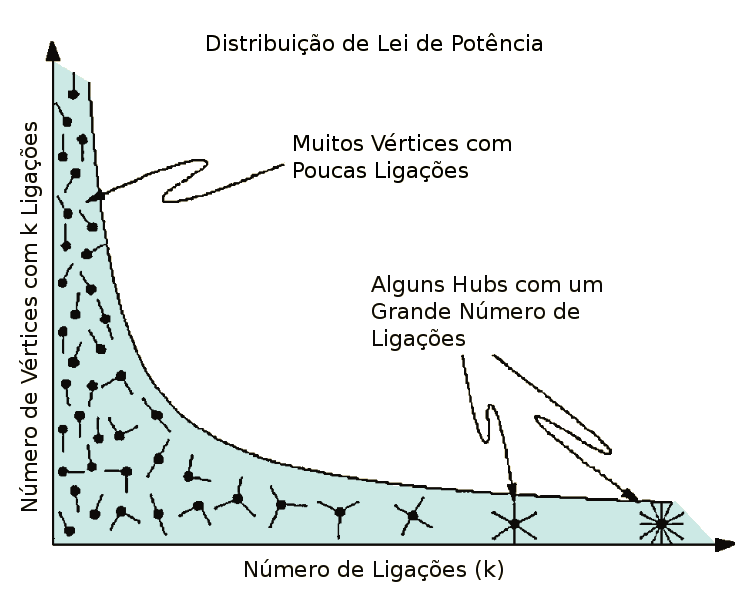
\includegraphics[width=0.5\textwidth]{leidepotencia}
\caption{Distribuição de graus como lei de potência. Adaptado de \cite{Barabasi2007}.}
\end{figure}

Esse resultado foi considerado surpreendente, pois contradiz a hipótese de que redes reais obedecem ao modelo de Erdős-Rényi \cite{Erdos1959}, também chamado de modelo de rede aleatória. Nesse modelo, a probabilidade de um par de vértices ser ligado por uma aresta é constante e igual a $p$. Demonstra-se que a distribuição dos graus de redes geradas por esse modelo é bem aproximada pela distribuição de Poisson.

Uma característica das redes livres de escala é a presença de vértices cujo grau é muito maior do que a média (informalmente chamados de \textit{hubs}). No caso de redes de Erdős-Rényi a probabilidade de existir um vértice com um determinado grau $k$ cai exponencialmente à medida que $k$ se afasta do valor médio e, por essa razão, nessas redes os vértices possuem mais ou menos o mesmo grau e a existência de \textit{hubs} é altamente improvável.

Barabási e Albert propuseram um modelo para explicar a formação das redes com distribuição de graus livre de escala, formado por dois mecanismos: crescimento contínuo e ligação preferencial. O modelo propõe que as redes crescem um vértice por vez e cada novo vértice se liga a um número fixo de vértices antigos, dando preferência aos vértices com maior grau (mais formalmente, a probabilidade de um vértice receber uma aresta é proporcional ao seu grau). Hoje sabe-se que redes livres de escala também podem ser geradas por outros modelos \cite{Albert2000,Kumar2000,Aiello2000b,Dorogovtsev2002,Bollobas2003,Deo2005}.

% Cada vértice em um grafo é caracterizado por um grau, k, que representa a quantidade de arestas ligadas a ele. No caso de grafos orientados, existe a distinção entre grau de saída e grau de entrada, que representam a quantidade de arcos que saem ou entram, respectivamente, do vértice.

\subsubsection{Efeito Mundo Pequeno}

A distância entre dois vértices de uma rede é o número de arestas do menor caminho que conecta os vértices. Diz-se que uma rede apresenta o efeito mundo pequeno quando a distância entre dois vértices é, em média, pequena, mesmo quando a rede é grande. Mais formalmente, a distância média entre vértices é proporcional ao logaritmo do número de vértices \cite{Watts1998}. Esse efeito foi detectado em diversas redes reais.

%Demonstra-se que tanto os grafos gerados pelo modelo de Erdős-Rényi quanto aqueles gerados pelo modelo de Barabási-Albert possuem essa propriedade.

% Nesse modelo os vértices são dispostos em uma circunferência e então cada vértice se conecta a um número fixo de vértices mais próximos. O grafo resultante é regular, isto é, todos os seus vértices possuem o mesmo grau. A seguir são criadas arestas entre pares de vértices escolhidos aleatoriamente. Essas arestas criam atalhos na rede e fazem com que a rede tenha a propriedade de mundo pequeno. // Rewire

\subsubsection{Coeficiente de agrupamento}

Os vizinhos de um vértice são todos os vértices com os quais ele compartilha uma aresta. O coeficiente de agrupamento de um vértice, $C_i$, é a fração de todos os possíveis pares de vizinhos do vértice que estão ligados por uma aresta, e é dado pela seguinte expressão:

\[  C_i = \frac{2x}{k_i(k_i - 1)} \]

onde $x$ é o número de pares de vizinhos do vértice $i$ que estão ligados por uma aresta e $k_i$ é o grau do vértice $i$ \cite{Watts1998}. Por definição, $C_i = 0$ quando $k_i < 2$. Define-se o coeficiente de agrupamento de um grafo, $C$, como a média aritmética dos coeficientes de agrupamento dos seus vértices. Demonstra-se que o coeficiente de agrupamento de uma rede aleatória de Erdős-Rényi é igual a $\langle k \rangle / n$ (onde $\langle k \rangle$ é o grau médio). Muitas redes complexas possuem um coeficiente de agrupamento alto, isto é, muito maior do que o coeficiente das redes aleatórias.

Outra característica observada em algumas redes é que o coeficiente de agrupamento de um vértice é inversamente proporcional ao grau do vértice, ou seja, $C(k) \sim k^{-1}$. Segundo Ravasz e Barabási \cite{Ravasz2003}, isso indica a existência de uma organização hierárquica na rede.

\subsubsection{Motivos}

Motivos são padrões de vértices e arestas que ocorrem com frequência em uma rede \cite{Milo2002}. Estudos recentes encontraram em redes de dependências entre componentes motivos presentes em redes de neurônios e em circuitos eletrônicos \cite{Valverde2005,Ma2008}. Especula-se que a formação de motivos em sistemas de \textit{software} seja resultado de restrições de custo e otimização impostas a sua evolução.

% \subsubsection{Assortatividade, mixing}

\subsubsection{Detecção de Comunidades}

Métricas globais como a distribuição de graus escondem o fato de que muitas redes se organizam em grupos de vértices relativamente independentes uns dos outros, chamados de comunidades. Detecção de comunidades é a tarefa de particionar os vértices de uma rede em comunidades de modo que, sob algum critério, os vértices de uma mesma comunidade estão fortemente relacionados entre si e fracamente relacionados a vértices de outras comunidades.

A detecção de comunidades é análoga ao que, na mineração de dados, se chama de análise de clustering --- sendo cluster, nesse contexto, sinônimo de comunidade. No domínio da engenharia de sofware, muitas técnicas de recuperação de arquitetura utilizam algoritmos de clustering para identificar módulos de um sistema de software.

A avaliação de algoritmos de clustering (ou detecção de comunidades) consiste em executar o algoritmo sobre uma rede cuja estrutura de clusters (ou comunidades) é conhecida e então comparar, através de alguma métrica, essa estrutura com a estrutura encontrada pelo algoritmo. Infelizmente não há muitas redes cuja estrutura de comunidades é conhecida, e as que existem são pequenas. Testes mais extensivos podem ser realizados com redes geradas por computador.

Newman e Girvan \cite{Newman2004a} propuseram um modelo que gera redes com 128 vértices, divididos em quatro comunidades de 32 vértices cada. Os vértices possuem aproximadamente o mesmo número de arestas, 16, das quais $z_{out}$ arestas ligam vértices de comunidades distintas. Newman e Girvan geraram redes com diferentes valores de $z_{out}$ com a finalidade de comparar dois algoritmos de detecção de comunidade.

Esse modelo possui algumas limitações: os vértices possuem aproximadamente o mesmo número de arestas, as comunidades possuem o mesmo tamanho e a rede é pequena. Com base nessa observação, Lancichinetti et al. \cite{Lancichinetti2008} propuseram um modelo no qual a distribuição de graus e a distribuição de tamanho das comunidades são ambas leis de potência e o número de vértices é arbitrário. Cada vértice compartilha uma fração constante de suas arestas com vértices de outras comunidades; essa fração é controlada pelo parâmetro de mistura, $\mu$.

O modelo de Lancichinetti et al. possui características que, a depender do domínio modelado, são pouco realistas: as redes são não-orientadas; todos os vértices possuem ligações tanto para vértices da mesma comunidade quanto para vértices de outras comunidades; todas as comunidades estão, potencialmente, ligadas a todas as outras.

% the preferred formulation of communities is often domain-specific.

\section{Redes de Dependências entre Componentes como Redes Complexas}

Estudos recentes têm aplicado a teoria das redes complexas em redes de dependências entre componentes de \textit{software}. Valverde e Solé \cite{Valverde2003} detectaram distribuições de graus livres de escala e alto coeficiente de agrupamento em redes não-orientadas formadas por relações de agregação de tipos em diagramas UML, programas em C e programas em C++. Myers \cite{Myers2003} analisou redes de chamadas de função em programas em C e redes de agregação e herança em programas em C++, modeladas como grafos orientados. Em ambos os casos ele identificou organização hierárquica através da distribuição do coeficiente de agrupamento, $C(k) \sim k^{-1}$. O estudo revelou ainda uma correlação negativa entre o grau de entrada e o grau de saída de um vértice. Leis de potência foram encontradas em trechos das distribuições de graus de entrada e das distribuições de graus de saída.

Distribuições de graus livres de escala também foram encontradas em programas escritos em Smalltalk \cite{Marchesi2004,Concas2007} e em Java \cite{Hyland-Wood2006,Baxter2006,Ichii2008}, em dependências entre pacotes de \textit{software} \cite{Labelle2004}, em chamadas de sistema, em dependências entre bibliotecas dinâmicas \cite{Louridas2008} e até mesmo em referências entre objetos em tempo de execução \cite{Potanin2005}.

É difícil comparar as pesquisas porque nem sempre elas deixam explícito que tipos de interação foram considerados para a construção das redes. Além disso, alguns trabalhos usam ferramentas estatísticas inadequadas para leis de potência.

%Nem todos os trabalhos usam a Estatística rigorosamente. Lognormal, double pareto, power law, stretched exponential, power law with exponential cutoff... Alguns usam o coeeficiente de determinação ($R^2$), que não se aplica a leis de potência, ou o método dos mínimos quadrados sobre o logaritmo dos dados.

\section{Tratamento Estatístico de Leis de Potência} \label{sec:estatistica}

\subsection{Histograma}

A estratégia mais usada para determinar se um conjunto de dados segue uma lei de potência é plotar o seu histograma em escala log-log. Se os dados seguem a lei de potência, o gráfico resultante deve ser uma reta. No entanto alguns cuidados precisam ser tomados ao traçar o histograma.

Quando o histograma agrupa os dados em classes de mesmo tamanho, o gráfico apresenta muito ruído na cauda, na região onde se encontram os maiores valores, como mostra a Figura \ref{fig:histogramas}(b). Isso ocorre porque nessa região os dados são esparsos, já que a probabilidade é baixa.

Uma maneira de reduzir o ruído consiste em agrupar os dados em classes cujo tamanho cresce exponencialmente. Por exemplo, podemos considerar classes formadas pelos intervalos de 1 a 2, de 2 a 4, de 4 a 8, de 8 a 16, e assim sucessivamente. A contagem de amostras de uma classe, nesse caso, deve ser dividida pelo tamanho do intervalo, a fim de normalizar o histograma \cite{Newman2005}. Note como o ruído foi reduzido na Figura \ref{fig:histogramas}(c).

Uma solução um pouco diferente é traçar o gráfico da função de distribuição cumulativa complementar (fdcc). Essa função representa, para cada valor $x$, o número de elementos com valor maior do que $x$. Não há necessidade de dividir os dados em classes. Se os dados seguem uma lei de potência com expoente $\gamma$, sua fdcc será uma lei de potência com expoente $\gamma – 1$. O gráfico é mostrado na Figura \ref{fig:histogramas}(d).

\begin{figure} \label{fig:histogramas}
\centering
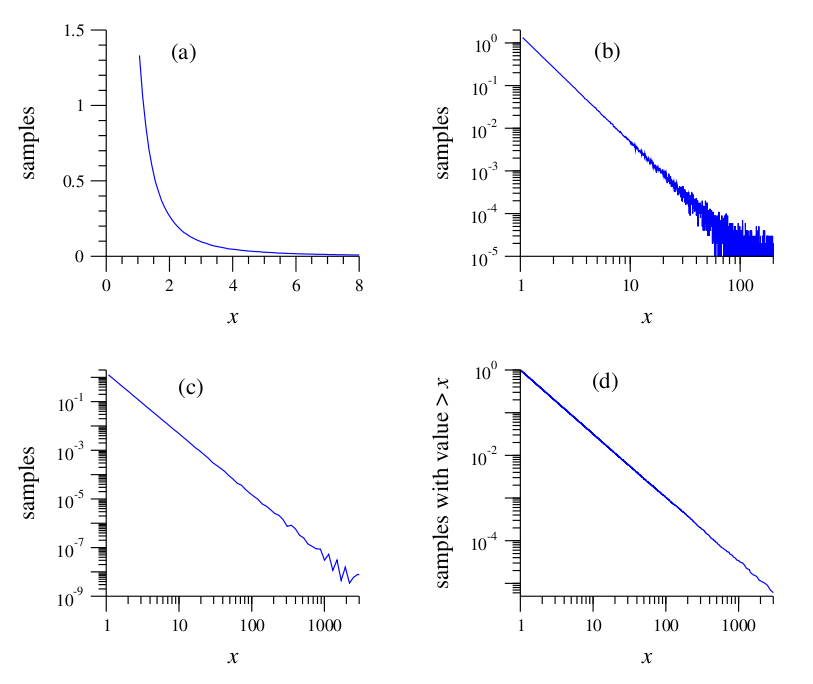
\includegraphics[width=0.7\textwidth]{histogramas}
\caption{(a) Histograma de um conjunto de 1 milhão de números aleatórios, com distribuição de lei de potência com $\gamma = 2,5$. (b) O mesmo histograma, em escala log-log. (c) Histograma construído com classes de tamanho exponencial. (d) A função de distribuição cumulativa complementar do mesmo conjunto de dados. Fonte: \cite{Newman2005}.}
\end{figure}

% TODO: inserir figura do artigo de Newman.

\subsection{Estimação de Parâmetros}

Poucos dados empíricos seguem uma lei de potência em toda a sua extensão. Normalmente a lei de potência se aplica apenas a valores maiores do que um valor mínimo, $x_{min}$, e nesse caso se diz que a cauda da distribuição segue uma lei de potência. O parâmetro $x_{min}$ pode ser estimado visualmente através da observação do histograma ou através de métodos estatísticos \cite{Clauset2007}.

Ao extrair o logaritmo da lei de potência, obtemos $\log(p(k)) \sim -\gamma \log(k)$, que é uma reta com coeficiente angular $-\gamma$. Por essa razão uma técnica comum para estimar o parâmetro $\gamma$ de um conjunto de dados consiste em aplicar o método dos mínimos quadrados sobre o logaritmo dos dados a fim de encontrar o coeficiente angular da reta. Esse método, no entanto, introduz erros sistemáticos no caso da lei de potência, e por isso recomenda-se o uso do método da máxima verossimilhança \cite{Clauset2007}. O 

\subsection{Teste de Ajustamento}

Estimados os parâmetros $x_{min}$ e $\gamma$, convém verificar se os dados se ajustam bem a uma lei de potência. Um valor alto para o coeficiente de determinação, $R^2$, não é suficiente para afirmar que o ajuste é bom. Uma  forma melhor de realizar a verificação consiste em gerar leis de potência com os parâmetros estimados e compará-las aos dados através do teste de ajustamento de Kolmogorov-Smirnov. Para um maior rigor, é preciso ajustar outras distribuições teóricas aos dados e verificar qual se ajusta melhor.

A depender da aplicação pode não ser importante determinar se a distribuição dos dados segue perfeitamente uma lei de potência. Em muitos casos é suficiente observar que os dados são distribuídos de forma bastante heterogênea, formando uma cauda pesada, que decai lentamente.

%%%%%%%%%%%%%%%%%%%%%%%%%%%%%%%%%%%%%%%%%%%%%%%%%%%%%%%%%%%%%%%%%%%%%%%%%%%%%%%%%%%%%%%%%%%%%%%
%%%%%%%%%%%%%%%%%%%%%%%%%%%%%%%%%%%%%%%%%%%%%%%%%%%%%%%%%%%%%%%%%%%%%%%%%%%%%%%%%%%%%%%%%%%%%%%
%%%%%%%%%%%%%%%%%%%%%%%%%%%%%%%%%%%%%%%%%%%%%%%%%%%%%%%%%%%%%%%%%%%%%%%%%%%%%%%%%%%%%%%%%%%%%%%
%%%%%%%%%%%%%%%%%%%%%%%%%%%%%%%%%%%%%%%%%%%%%%%%%%%%%%%%%%%%%%%%%%%%%%%%%%%%%%%%%%%%%%%%%%%%%%%

% Modelos: Bollobas, Deo and Cami

%%%%%%%%%%%%%%%%%%%%%%%%%%%%%%%%%%%%%%%%%%%%%%%%%%%%%%%%%%%%%%%%%%%%%%%%%%%%%%%%%%%%%%%%%%%%%%%
%%%%%%%%%%%%%%%%%%%%%%%%%%%%%%%%%%%%%%%%%%%%%%%%%%%%%%%%%%%%%%%%%%%%%%%%%%%%%%%%%%%%%%%%%%%%%%%
%%%%%%%%%%%%%%%%%%%%%%%%%%%%%%%%%%%%%%%%%%%%%%%%%%%%%%%%%%%%%%%%%%%%%%%%%%%%%%%%%%%%%%%%%%%%%%%


% \section{Recuperação de Arquitetura}
% 
% \subsection{Arquitetura: Componentes e Conectores}
% 
% Componentes e conectores.
% Visões. Processos, módulos.
% 
% \subsection{Técnicas de Recuperação de Arquitetura}
% 
% 
% Análise dinâmica, análise estática. Padrões de nomes (Anquetil). Padrões estrutrais (LIMBO). Análise de clustering (Maqbool)
% 
% 
% 
% Sobre clustering. Referência: Introduction to Data Mining, capítulo 8



% \subsection{Tipos de Decomposições}
% 
% Referência: Introduction to Data Mining, capítulo 8 \cite{Tan2005}
% 
% Hierárquica vs partitiva.
% Exclusive vs overlapping vs fuzzy.
% Completa vs. parcial.
% 
% \subsection{Algoritmos}
% 
% Bunch. LIMBO. MCL etc. (a escolher)
% 
% \subsection{Avaliação de Decomposições}
% 
% Avaliação não-supervisionada: NED, estabilidade.
% Avaliação supervisionada: authoritativeness.
% 
% Avaliações relativas (comparar dois algoritmos)
% 
% \subsection{Comparação entre Decomposições}
% 
% Precision-recall.
% MoJo.
% EdgeMoJo.
% etc.

\bibliographystyle{alpha}
\bibliography{complex-networks,rodrigo-mestrado}

\end{document}

% Propriedades estatísticas da lei de potência. A Figura 1(a) mostra o gráfico de uma lei de potência. Intuitivamente, percebe-se que a grande maioria dos vértices possui um grau pequeno, mas existem vértices cujo grau está muito acima do grau médio. Trata-se de uma curva assimétrica positiva, pois a média é maior do que a mediana. A probabilidade de um elemento de grau alto é pequena mas não desprezível, e isso contribui para elevar a média. Como a distribuição é muito heterogênea, a média não é um valor muito representantivo da distribuição. A lei de potência, quando plotada em escala log-log, se apresenta sob a forma de uma reta. Dificilmente dados obtidos experimentalmente formam uma reta em toda sua extensão. Portanto muitas vezes quando se afirma que uma distribuição é livre de escala, o que se quer dizer é que parte da distribuição é bem aproximada por uma reta na escala log-log.

% As métricas citadas analisam propriedades de vértices isoladamente, como o coeficiente de agrupamento, estruturas compostas por pequenos conjuntos de vértice, os motivos, e propriedades globais, como a distribuição de graus. Existem ainda estruturas intermediárias, as comunidades. Uma comunidade é um subconjunto dos vértices de uma rede que são densamente conectados entre si e pouco conectados ao resto da rede \cite{Gulbahce2008}. As diversas comunidades de uma rede podem possuir características diversas, que não são evidenciadas por análises da estrutura global da rede. Muitas vezes se considera que comunidades representam módulos funcionais de uma rede --- uma comunidade seria, portanto, um conjunto de vértices similares, que interagem a fim de realizar uma funcionalidade.

% Muitas vezes a organização funcional dos vértices de uma rede é desconhecida, então se usam algoritmos que procuram detectar comunidades. Esses algoritmos fornecem um particionamento dos vértices de modo que cada partição corresponde a uma comunidade.

% Naturalmente, não existe uma definição formal e universalmente aceita do que é uma comunidade ou do que é um particionamento ótimo. 

% definição de cluster: A number of similar things collected together or lying contiguous; a group;

%A community is a densely connected subset of nodes that is only sparsely linked to the remaining network. (Gulbahce)

%Communities in a citation network might represent related papers on a single topic;

